\documentclass[border=3pt]{standalone}
% Preâmbulo compartilhado pelos diagramas TikZ da aula 9 de IHR (Robôs na Sociedade)
\usepackage[T1]{fontenc}
\usepackage[utf8]{inputenc}
\usepackage{lmodern}
\usepackage{amsmath}
\usepackage{xcolor}
\usepackage{tikz}
\usetikzlibrary{arrows.meta,angles,quotes,decorations.pathmorphing,decorations.pathreplacing,calc,
                positioning,shapes.geometric,shapes.misc,backgrounds,fit,
                math}

% Paleta (mesma dos SVGs originais)
% Paleta da disciplina de IHR: acento azul (#1A6FB5), cor de destaque do tema.
% (o nome "dblue" é mantido para não alterar todos os diagramas)
\definecolor{dblue}{HTML}{1A6FB5}
\definecolor{dorange}{HTML}{B3541E}
\definecolor{dgreen}{HTML}{4A7C59}
\definecolor{dred}{HTML}{9C4B4B}
\definecolor{dcream}{HTML}{F4F1EA}
\definecolor{dshade}{HTML}{DDD7C9}

% Função gaussiana (não normalizada por padrão de escala visual)
\pgfmathdeclarefunction{gauss}{3}{%
  \pgfmathparse{1/(#3*sqrt(2*pi))*exp(-((#1-#2)^2)/(2*#3^2))}%
}

% Estilos comuns (prefixo d... para não colidir com chaves internas do pgf)
\tikzset{
  >={Stealth[length=2mm]},
  dguide/.style={gray!55, dashed, line width=0.4pt},
  daxis/.style={gray!60, line width=0.7pt, ->},
  dbody/.style={fill=black!3, draw=black!80, line width=1pt},
  dacc/.style={draw=dblue, line width=1pt},
  dlbl/.style={black!55, font=\small},
  dsub/.style={black!45, font=\footnotesize},
  dstate/.style={circle, draw=black!80, fill=dcream, line width=1pt,
                 minimum size=17mm, font=\large, inner sep=1pt},
  dobs/.style={circle, draw=black!80, fill=dshade, line width=1pt,
               minimum size=14mm, font=\large, inner sep=1pt},
  dbox/.style={rounded corners=2pt, draw=black!80, fill=dcream, line width=1pt,
               align=center, inner sep=6pt},
  dop/.style={circle, draw=black!80, fill=white, line width=1pt,
              minimum size=6mm, inner sep=0pt, font=\small},
  dtrans/.style={->, dblue, line width=1pt},
  dmeas/.style={->, dorange, line width=1pt},
  dcurve/.style={line width=1pt, dblue},
  dcurveb/.style={line width=1.4pt, dorange},
}

\begin{document}
\hyphenpenalty=10000 \exhyphenpenalty=10000 \tolerance=9999 \emergencystretch=3em
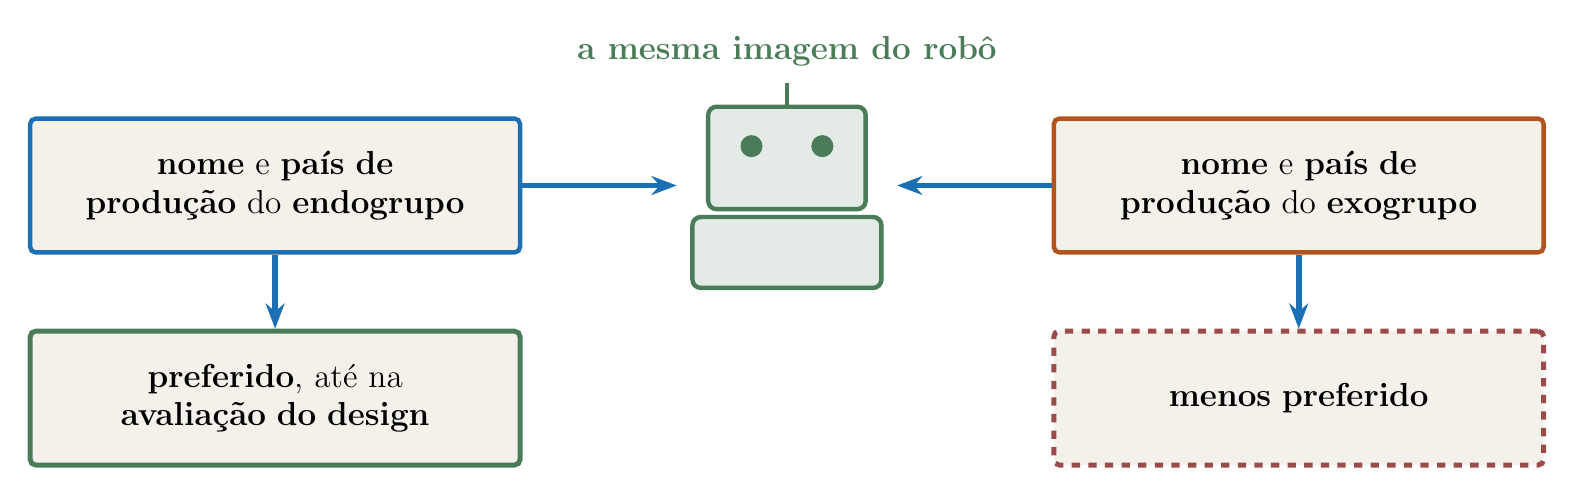
\begin{tikzpicture}[x=1cm,y=1cm]
\tikzset{k/.style={dbox, text width=5.8cm, minimum height=1.7cm, font=\large, line width=1.6pt}}
\draw[dgreen, fill=dgreen!15, line width=1.6pt, rounded corners=3pt] (8.7,3.0) rectangle (10.7,4.3);
\fill[dgreen] (9.25,3.8) circle (0.14); \fill[dgreen] (10.15,3.8) circle (0.14);
\draw[dgreen, line width=1.6pt] (9.7,4.3) -- (9.7,4.6);
\draw[dgreen, fill=dgreen!15, line width=1.6pt, rounded corners=3pt] (8.5,2.0) rectangle (10.9,2.9);
\node[font=\large\bfseries, dgreen] at (9.7,5.0) {a mesma imagem do robô};
\node[k, draw=dblue] (a) at (3.2,3.3) {\textbf{nome} e \textbf{país de produção} do \textbf{endogrupo}};
\node[k, draw=dorange] (b) at (16.2,3.3) {\textbf{nome} e \textbf{país de produção} do \textbf{exogrupo}};
\draw[dtrans, line width=2pt, -{Stealth[length=3.2mm]}] (a.east) -- (8.3,3.3);
\draw[dtrans, line width=2pt, -{Stealth[length=3.2mm]}] (b.west) -- (11.1,3.3);
\node[k, draw=dgreen, line width=1.8pt] (c) at (3.2,0.6) {\textbf{preferido}, até na \textbf{avaliação do design}};
\node[k, draw=dred, dashed, line width=1.8pt] (d) at (16.2,0.6) {\textbf{menos preferido}};
\draw[dtrans, line width=2pt, -{Stealth[length=3.2mm]}] (a.south) -- (c.north);
\draw[dtrans, line width=2pt, -{Stealth[length=3.2mm]}] (b.south) -- (d.north);
\end{tikzpicture}
\end{document}
